
\newcommand{\xxtheta}{f_\theta} 
\section{问题陈述与背景}
\label{sec:background}

我们首先定义可控生成（\cref{ssec:control_setup}），随后回顾连续扩散模型（\cref{ssec:diffusion_setup}）。

\subsection{文本生成模型与可控生成} 
\label{ssec:control_setup}
文本生成的任务是从已训练的语言模型 $\plm (\ww)$ 中采样 $\ww$，其中 $\ww = [w_1 \cdots w_n]$ 是离散词序列，$\plm (\ww)$ 是词序列上的概率分布。可控文本生成的任务是从条件分布 $p(\ww \mid \cc)$ 中采样 $\ww$，其中 $\cc$ 表示一个\emph{控制}变量。对于句法控制，$\cc$ 可以是目标句法树（\cref{fig:1}）；对于情感控制，$\cc$ 可以是期望的情感标签。可控生成的目标是生成满足控制目标 $\cc$ 的 $\ww$。

考虑 plug-and-play 可控生成设定：给定一个由大量无标注文本数据训练得到的语言模型 $\plm(\ww)$，并且对于每个控制任务，给定一个由较少量有标注文本数据训练得到的分类器 $p(\cc \mid \ww)$（例如，对于句法控制，该分类器是概率解析器）。目标是利用这两个模型，通过 Bayes 规则 $p(\ww \mid \cc) \propto \plm(\ww) \cdot p(\cc \mid \ww)$ 从后验 $p(\ww \mid \cc)$ 中近似采样。这里，$\plm(\ww)$ 鼓励 $\ww$ 保持流畅，而 $p(\cc \mid \ww)$ 鼓励 $\ww$ 满足控制。






\subsection{自回归语言模型}
语言建模的典型方法以从左到右的自回归方式分解 $\plm$，即 $\plm(\ww) = \plm(w_1) \prod_{i=2}^n \plm(x_i \mid x_{<i})$。在这种情况下，文本生成被化约为在已生成部分序列条件下反复预测 next-token 的任务。next-token 预测 $\plm(x_i \mid x_{<i})$ 通常由 Transformer 架构 \cite{Vaswani2017Attn} 参数化。

\subsection{连续域的扩散模型}
\label{ssec:diffusion_setup}

扩散模型 \citep{ho2020denoising,nichol2021improved} 是一种隐变量模型，它将数据 $\cx{0} \in \mathbb{R}^d$ 建模为 Markov 链 $\cx{T} \dots \cx{0}$，其中每个变量都在 $\mathbb{R}^d$ 中，且 $\cx{T}$ 是 Gaussian。扩散模型逐步对隐变量序列 $\cx{T:1}$ 去噪，以近似来自目标数据分布的样本~（\cref{fig:graphical_model}）。初始状态 $p_\theta(\cx{T}) \approx \mathcal{N} (0, \mathbf{I})$，每个去噪转移 $\cx{t} \rightarrow \cx{t-1}$ 由模型 $\ptheta(\cx{t-1}\mid \cx{t}) = \mathcal{N}(\cx{t-1}; \mu_\theta(\cx{t}, t), \Sigma_\theta(\cx{t}, t))$ 参数化。例如，$\mu_\theta$ 和 $\Sigma_\theta$ 可由 U-Net 或 Transformer 计算得到。


为了训练扩散模型，我们定义一个构造中间隐变量 $\cx{1:T}$ 的前向过程。前向过程逐步向数据 $\cx{0}$ 添加 Gaussian 噪声，直到在扩散步骤 $T$ 时样本 $\cx{T}$ 近似为 Gaussian。每个转移 $\cx{t-1} \rightarrow \cx{t}$ 由 $q(\cx{t} \mid \cx{t-1}) = \mathcal{N} (\cx{t} ; \sqrt{1-\beta_t} \cx{t-1}, \beta_t \mathbf{I})$ 参数化，其中超参数 $\beta_t$ 是扩散步骤 $t$ 添加的噪声量。
前向过程 $q$ 的这种参数化不包含可训练参数，并使我们能够定义一个训练目标：按照预定义的前向过程 $q$ 生成带噪数据，并训练模型反转该过程以重构数据。




\begin{figure}
    \centering
    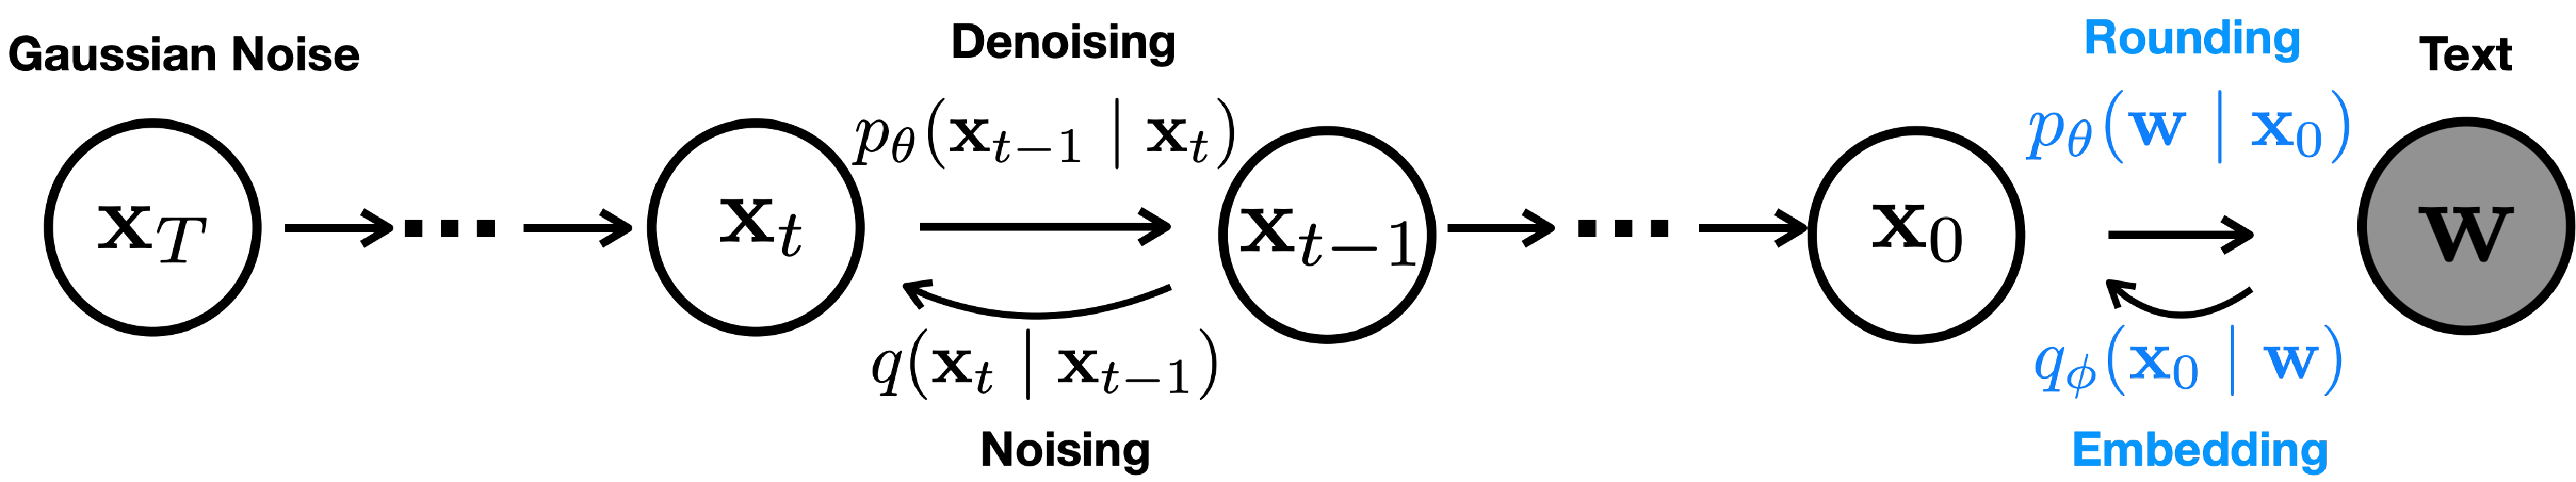
\includegraphics[width=0.8\textwidth]{fig/graphical_model_v2.pdf}
    \caption{\label{fig:graphical_model} 表示前向和反向扩散过程的图模型。除原始扩散模型 \cite{ho2020denoising} 外，我们在 $\cx{0}$ 与 $\ww$ 之间加入一个 Markov 转移，并提出 embedding \cref{ssec:embeddings} 和 rounding \cref{ssec:rounding} 技术。}
    \vspace{-5mm}
\end{figure}

扩散模型通过最大化数据的边际似然 $\mathbb{E}_{\cx{0} \sim p_\text{data} }[\log p_\theta(\cx{0})]$ 进行训练，其典型目标是 $\log p_\theta(\cx{0})$ 的变分下界 \cite{pmlr-v37-sohl-dickstein15}，
\begin{equation}
\Lvlb (\cx{0}) = \mathop{\mathbb{E}}_{q(\cx{1:T} | \cx{0})} \left[\log \frac{q(\cx{T} | \cx{0})}{\ptheta(\cx{T})} + \sum_{t=2}^T \log \frac{q(\cx{t-1} | \cx{0},\cx{t})} {\ptheta(\cx{t-1} | \cx{t}) } - \log \ptheta( \cx{0} | \cx{1})\right].
\label{eqn:diffusion}
\end{equation}
然而，该目标可能不稳定，并且需要许多优化技巧来稳定训练 \cite{nichol2021improved}。为规避这一问题，\citet{ho2020denoising} 设计了一个简单的替代目标，对 $\Lvlb$ 中每个 KL-divergence 项进行展开并重新加权，从而得到均方误差损失（推导见 \cref{app:derive}），我们将其记为
\[\Lsimple (\cx{0}) = \sum_{t=1}^T \mathop{\mathbb{E}}_{q(\cx{t} \mid \cx{0})} || \mu_\theta(\cx{t}, t) - \hat{\mu}(\cx{t}, \cx{0}) ||^2,\]
其中 $\hat{\mu}(\cx{t}, \cx{0})$ 是后验 $q(\cx{t-1} | \cx{0},\cx{t})$ 的均值，该后验是闭式 Gaussian；$\mu_\theta(\cx{t}, t)$ 是由神经网络计算得到的 $\ptheta(\cx{t-1} \mid \cx{t})$ 的预测均值。
虽然 $\Lsimple$ 不再是有效下界，但先前工作发现它在经验上使训练更稳定并提高了样本质量\footnote{我们这里对 $\Lsimple$ 的定义使用了与 \citet{ho2020denoising} 不同的参数化。我们用 $\mu_\theta(\cx{t}, t)$ 表示平方损失，而他们用 $\epsilon_\theta(\cx{t}, t)$ 表示。}。
我们将在 Diffusion-LM 中使用类似的简化，以稳定训练并提升样本质量（\cref{ssec:embeddings}）。














\vspace{-2mm}
\section{Diffusion-LM：连续扩散语言建模}
\vspace{-2mm}
\label{sec:method}

构建 Diffusion-LM 需要对标准扩散模型进行若干修改。
首先，我们必须定义一个 embedding 函数，将离散文本映射到连续空间。为此，我们提出一个用于学习 embeddings 的端到端训练目标（\cref{ssec:embeddings}）。
其次，我们需要一种 rounding 方法，将 embedding 空间中的向量映射回词。为此，我们提出训练和解码阶段的方法以促进 rounding（\cref{ssec:rounding}）。








\vspace{-2mm}
\subsection{端到端训练} 
\label{ssec:embeddings}


为将连续扩散模型应用于离散文本，我们定义 embedding 函数 $\Emb(w_i)$，将每个词映射到 $\mathbb{R}^{d}$ 中的向量。我们将长度为 $n$ 的序列 $\ww$ 的 embedding 定义为：$\Emb(\ww) = [\Emb(w_1), \dots, \Emb(w_n)] \in \mathbb{R}^{nd}$。

我们提出对扩散模型训练目标（Equation \ref{eqn:diffusion}）的修改，以联合学习扩散模型的参数和词 embeddings。
在初步实验中，我们探索了随机 Gaussian embeddings 以及预训练词 embeddings \cite{pennington-etal-2014-glove, radford2019language}。我们发现，与端到端训练相比，这些固定 embeddings 对 Diffusion-LM 而言是次优的\footnote{尽管可训练 embeddings 在控制和生成任务上表现最佳，但我们发现，在优化 held-out 困惑度时，映射到词表单纯形上的固定 embeddings 是有帮助的。由于本文关注生成质量而非困惑度，我们将该方法与困惑度结果的讨论留到 \cref{app:simplex}。}。


如 Figure \ref{fig:graphical_model} 所示，我们的方法在前向过程中加入从离散词 $\ww$ 到 $\cx{0}$ 的 Markov 转移，由 $\qphi(\cx{0} | \ww) = \mathcal{N} (\Emb(\ww), \sigma_0 I )$ 参数化。在反向过程中，我们加入一个可训练的 rounding 步骤，由 $\ptheta(\ww \mid \cx{0}) = \prod_{i=1}^n \ptheta(w_i \mid x_i)$ 参数化，其中 $\ptheta(w_i \mid x_i)$ 是 softmax 分布。\cref{sec:background} 中引入的训练目标现在变为
\begin{equation}
\begin{aligned}
\mathcal{L}^\text{e2e}_{\text{vlb}} (\ww) &= \mathop{\mathbb{E}}_{q_\phi(\cx{0} | \ww)}\left[\mathcal{L}_{\text{vlb}} (\cx{0}) + \log \qphi(\cx{0} | \ww) - \log \ptheta(\ww | \cx{0})]\right], \\
 \mathcal{L}^\text{e2e}_\text{simple} (\ww) &= \mathop{\mathbb{E}}_{\qphi(\cx{0:T} | \ww)} \left[\Lsimple(\cx{0}) + || \Emb(\ww) - \mu_\theta(\cx{1}, 1) ||^2  - \log \ptheta(\ww | \cx{0})\right].
\end{aligned}
\label{obj:e2e}
\end{equation}
\begin{wrapfigure}[11]{R}{0.5\textwidth}
\vspace{-10mm}
\centering
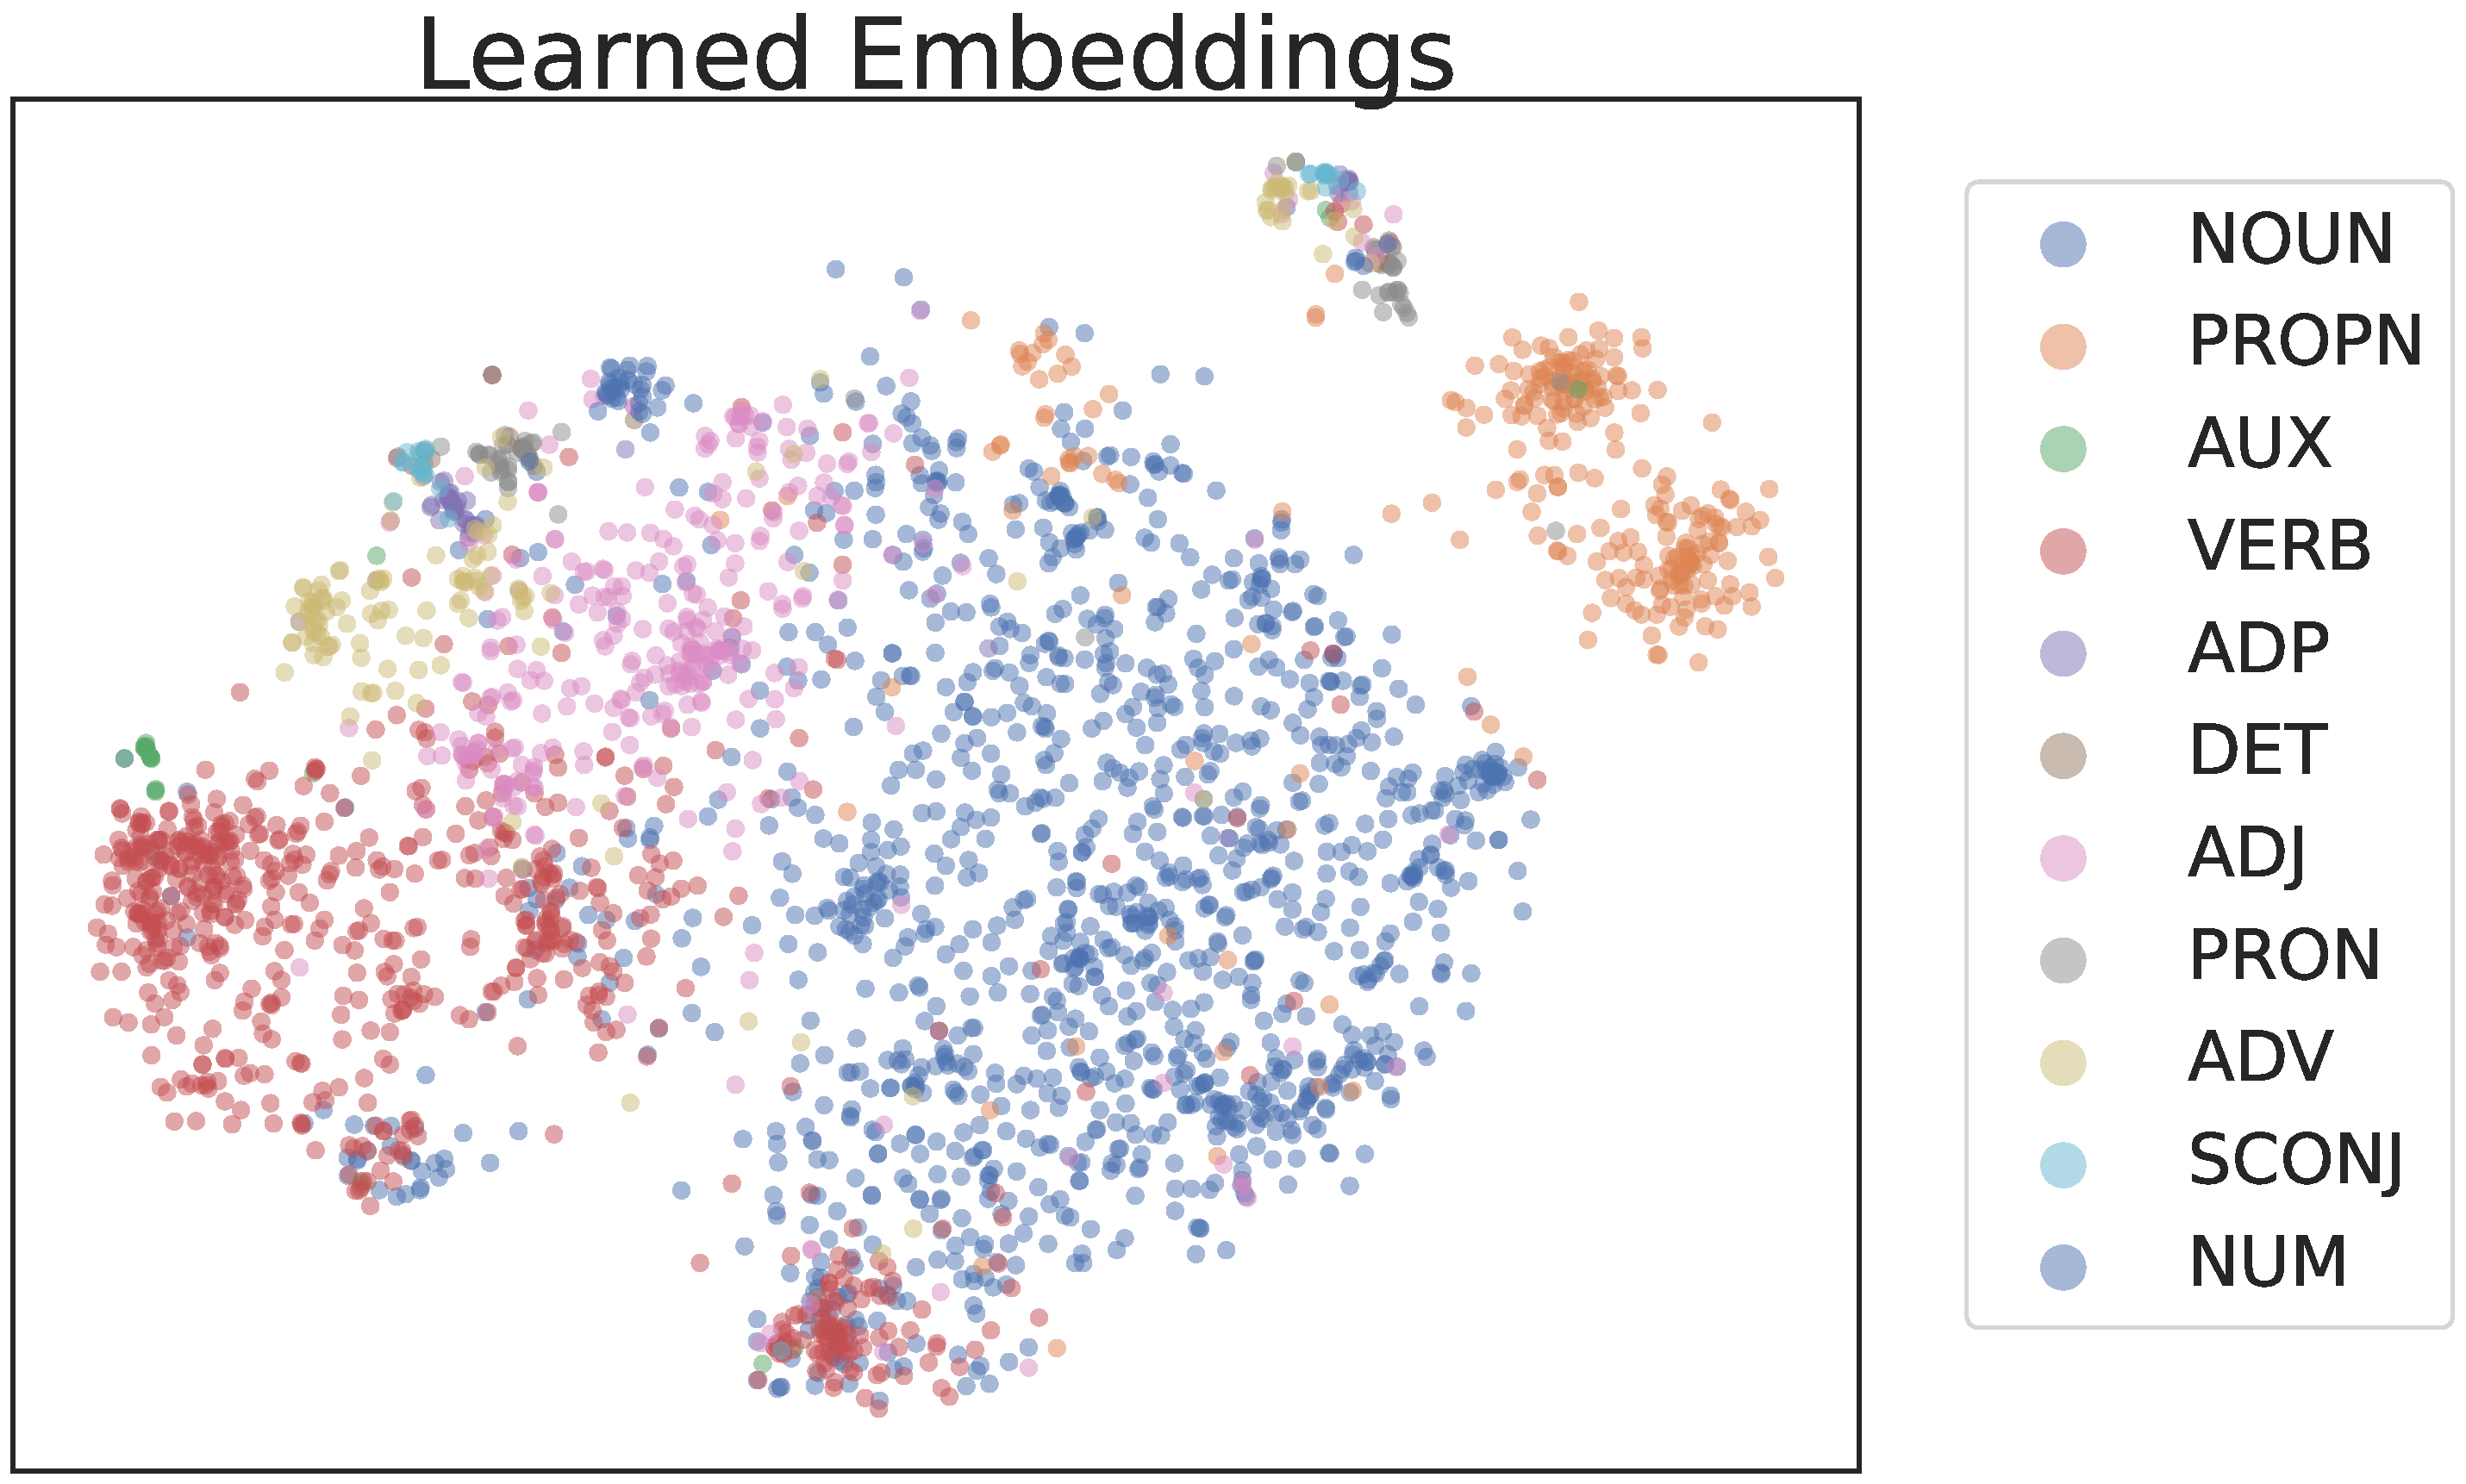
\includegraphics[width=\linewidth]{fig/embedding_128_v3.pdf}\caption{ \label{fig:emb} 学到的词 embeddings 的 t-SNE \cite{vanDerMaaten2008} 图。每个词按其 POS 着色。\looseness=-1 }
\end{wrapfigure}

我们遵循 \cref{ssec:diffusion_setup} 中的简化，从 $\mathcal{L}^\text{e2e}_{\text{vlb}}(\ww)$ 推导 $ \mathcal{L}^\text{e2e}_\text{simple} (\ww)$，推导细节见 \cref{app:derive}。由于我们正在训练 embedding 函数，$q_\phi$ 现在包含可训练参数，因此我们使用重参数化技巧 \citep{rezende2014stochastic, kingma2014auto} 通过该采样步骤进行反向传播。
经验上，我们发现学到的 embeddings 形成有意义的聚类：具有相同 part-of-speech 标签（句法角色）的词倾向于聚在一起，如 \cref{fig:emb} 所示。



\subsection{减少 Rounding 错误}
\label{ssec:rounding}


学到的 embeddings 定义了从离散文本到连续 $\cx{0}$ 的映射。我们现在描述其逆过程，即将预测的 $\cx{0}$ rounding 回离散文本。Rounding 通过根据 argmax $\ptheta(\ww \mid \cx{0})= \prod_{i=1}^n \ptheta(w_i \mid x_i)$ 为每个位置选择概率最高的词来实现。理想情况下，这种 argmax-rounding 足以映射回离散文本，因为去噪步骤应确保 $\cx{0}$ 精确落在某个词的 embedding 上。然而在经验上，模型无法生成承诺于单个词的 $\cx{0}$。



这一现象的一种解释是，我们目标 \ref{obj:e2e} 中的 $\Lsimple(\cx{0})$ 项对 $\cx{0}$ 结构建模的强调不足。回忆我们定义 $\Lsimple(\cx{0}) =\sum_{t=1}^T \mathbb{E}_{\cx{t}}|| \mu_\theta(\cx{t}, t) - \hat{\mu}(\cx{t}, \cx{0}) ||^2$，其中我们的模型 $\mu_\theta(\cx{t}, t)$ 在每个去噪步骤 $t$ 直接预测 $\ptheta(\cx{t-1}\mid \cx{t})$ 的均值。
在该目标中，$\cx{0}$ 必须承诺于单个词 embedding 的约束只会出现在 $t$ 接近 $0$ 的项中；我们发现，这种参数化需要仔细调参才能迫使目标强调这些项（见 \cref{app:ablation}）。


\newcommand{\Lsimplexx}{\mathcal{L}^\text{e2e}_{\cx{0}\text{-simple}}}
我们的方法对 $\Lsimple$ 重新参数化，迫使 Diffusion-LM 在目标的\emph{每一}项中显式建模 $\cx{0}$。具体而言，我们推导了一个通过 $\cx{0}$ 参数化的 $\Lsimple$ 类似形式，
$\Lsimplexx(\cx{0})=\sum_{t=1}^T \mathbb{E}_{\cx{t}} ||\xxtheta(\cx{t}, t) - \cx{0} ||^2$，其中我们的模型 $\xxtheta(\cx{t}, t)$ 直接预测 $\cx{0}$\footnote{预测 $\cx{0}$ 与预测 $\cx{t-1}$ 只相差缩放常数，因为 $\cx{t-1}$ 的分布可通过前向过程 $\cx{t-1} = \sqrt{\alphabar} \cx{0} +\sqrt{1-\alphabar} \epsilon$ 以闭式获得，更多细节见 \cref{app:derive}。}。这迫使神经网络在每一项中预测 $\cx{0}$，并且我们发现，用该目标训练的模型会很快学到 $\cx{0}$ 应精确地位于某个词 embedding 的中心。

我们已经说明重新参数化如何有助于模型训练，但我们也发现，同一直觉可在解码时用于一种称为\emph{clamping} 技巧的方法。
对于 $\cx{0}$-参数化模型的标准生成方法，模型先通过 $\xxtheta(\cx{t}, t)$ 计算 $\cx{0}$ 的估计，然后在该估计条件下采样 $\cx{t-1}$，从而将 $\cx{t}$ 去噪为 $\cx{t-1}$：$\cx{t-1} = \sqrt{\alphabar} \xxtheta(\cx{t}, t) +\sqrt{1-\alphabar} \epsilon$，其中 $\alphabar_t = \prod_{s=0}^t (1-\beta_s)$ 且 $\epsilon \sim \mathcal{N}(0,I)$\footnote{这来自边缘分布 $q(\cx{t} \mid \cx{0})$，由于所有 Markov 转移都是 Gaussian，该分布具有闭式形式。}。在 clamping 技巧中，模型还会将预测向量 $\xxtheta(\cx{t}, t)$ 映射到最近的词 embedding 序列。此时，采样步骤变为 $\cx{t-1} = \sqrt{\alphabar}\cdot \Clamp(\xxtheta(\cx{t}, t)) +\sqrt{1-\alphabar} \epsilon$。Clamping 技巧迫使预测向量在中间扩散步骤承诺于某个词，使向量预测更精确并减少 rounding 错误。\footnote{直观上，在 $t$ 接近 $T$ 的早期扩散步骤应用 clamping 技巧可能是次优的，因为模型尚未确定要承诺于哪些词。经验上，对所有扩散步骤应用 clamping 技巧不会显著损害性能。但遵循这一直觉，也可以将 clamping 技巧的起始步骤设为超参数。}
















\section{使用 Diffusion-LM 进行解码与可控生成}
\label{sec:decode}
在描述 Diffusion-LM 之后，我们现在考虑可控文本生成（\cref{ssec:control_text}）和解码（\cref{ssec:mbr1}）问题。


\subsection{可控文本生成}
\label{ssec:control_text}
我们现在描述一种在 Diffusion-LM 上实现 plug-and-play 控制的过程。我们的控制方法受到 \cref{ssec:control_setup} 中 Bayesian 形式化的启发，但并不直接在离散文本上进行控制，而是在 Diffusion-LM 定义的连续隐变量序列 $\cx{0:T}$ 上进行控制，并应用 rounding 步骤将这些隐变量转换为文本。

控制 $\cx{0:T}$ 等价于从后验 $p(\cx{0:T} | \cc) = \prod_{t=1}^T p(\cx{t-1} \mid \cx{t}, \cc)$ 解码，并且我们将该联合推理问题分解为每个扩散步骤上的一系列控制问题：$p(\cx{t-1} \mid \cx{t}, \cc) \propto p(\cx{t-1} \mid \cx{t}) \cdot p(\cc \mid \cx{t-1}, \cx{t})$。
进一步地，我们依据先前控制扩散工作的条件独立假设 \cite{song2021scorebased}，将 $p(\cc \mid \cx{t-1}, \cx{t})=p(\cc \mid \cx{t-1})$ 简化。因此，对于第 $t$ 步，我们在 $\cx{t-1}$ 上执行梯度更新：
\begin{align*}
    \nabla_{\cx{t-1}} \log p(\cx{t-1} \mid \cx{t}, \cc) = \nabla_{\cx{t-1}} \log p(\cx{t-1} \mid \cx{t}) + \nabla_{\cx{t-1}}  \log  p(\cc \mid \cx{t-1}),
\end{align*}
其中 $\log p(\cx{t-1} \mid \cx{t})$ 和 $\log p(\cc \mid \cx{t-1})$ 都是可微的：第一项由 Diffusion-LM 参数化，第二项由神经网络分类器参数化。


类似于图像设定中的工作 \cite{dhariwal2021diffusion,song2021scorebased}，我们在扩散隐变量上训练分类器，并在隐空间 $\cx{t-1}$ 上执行梯度更新，以引导其满足控制。这些图像扩散工作在每个扩散步骤沿 $\nabla_{ \cx{t-1}} \log  p(\cc \mid \cx{t-1})$ 方向走一步梯度。为提升文本上的性能并加速解码，我们引入两个关键修改：流畅性正则化和多步梯度更新。\looseness=-1




为生成流畅文本，我们在带有\emph{流畅性正则化}的控制目标上执行梯度更新：$ \lambda \log p(\cx{t-1} \mid \cx{t}) + \log p(\cc \mid \cx{t-1})$，其中 $\lambda$ 是在流畅性（第一项）与控制（第二项）之间权衡的超参数。尽管现有的扩散可控生成方法未在目标中包含 $\lambda \log p(\cx{t-1} \mid \cx{t})$ 项，我们发现该项对于生成流畅文本至关重要。所得可控生成过程可视为一种随机解码方法，它在最大化与采样 $p(\cx{t-1} \mid \cx{t}, \cc)$ 之间取得平衡，这很像 nucleus sampling~\cite{Holtzman2020Nucleus} 或低温采样等流行文本生成技术。为提升控制质量，我们对每个扩散步骤执行多步梯度更新：对每个扩散步骤运行 $3$ 步 Adagrad\footnote{我们尝试了将 Adagrad 替换为 SGD 的消融，但发现 Adagrad 对超参数调节明显不那么敏感。} \cite{Duchi2010AdaptiveSM} 更新。为缓解增加的计算成本，我们将扩散步骤从 2000 下采样到 200，这能加速我们的可控生成算法且不会显著损害样本质量。


\subsection{最小 Bayes 风险解码}
\label{ssec:mbr1}
许多条件文本生成任务需要一个\emph{单一}的高质量输出序列，例如机器翻译或句子 infilling。
在这些设定中，我们应用 Minimum Bayes Risk (MBR) 解码 \cite{kumar-byrne-2004-minimum} 来聚合从 Diffusion-LM 抽取的一组样本 $\mathcal{S}$，并选择在损失函数 $\mathcal{L}$（例如负 BLEU 分数）下达到最小期望风险的样本：$\hat{\ww} = \argmin_{\ww \in S} \sum_{\ww' \in S} \frac{1}{|S|}\mathcal{L}(\ww, \ww')$。我们发现 MBR 解码通常会返回高质量输出，因为低质量样本会与其余样本不相似，并受到损失函数惩罚。






